\section{Estado del arte}\label{sec:state_of_the_art}

\subsection{Simuladores de tráfico}

Actualmente, existe una gran oferta de simuladores de tráfico, ya sean de fuente abierta o propietarios. Ratrout y Rahman listan 14 de estos en su análisis comparativo del año 2009 \autocite{ratrout2009comparative}, mientras que Boxill y Yu, ya en el año 2000 presentaban 8 simuladores distintos en su estudio de simuladores para el desarrollo de Sistemas Inteligentes de Transporte \autocite{boxill2000evaluation}.

En esta sección se presentará brevemente el estado del arte de los más prominentes de estos simuladores, basándose en la revisión de literatura realizada por Mubasher y ul Qounain en \autocite{traffic_sim_review}.

\begin{table}
    \centering
    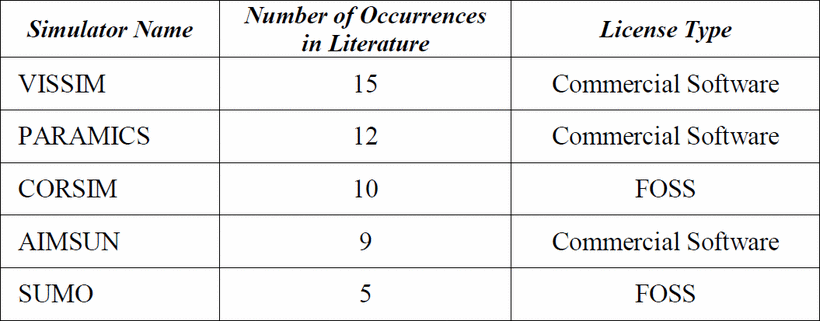
\includegraphics[width=\linewidth]{figuras/popular_trafficsims}
    \caption[Tabla comparativa simuladores de tráfico.]{Los cinco simuladores más prominentes en la literatura (fuente: Mubasher y ul Qounain \autocite{traffic_sim_review}).}
    \label{table:prom_trafficsim}
\end{table}

\subsubsection{VISSIM}

VISSIM es un entorno de simulación discreto y microscópico, desarrollado propietariamente por el Grupo PVT en Alemania \autocite{vissim}. Es un simulador generalista, capaz de modelar sistemas de transporte multi-modales, en los que interactúan tanto vehículos ``convencionales'' como bicicletas, tranvías y hasta trenes pesados \autocite{fellendorf2010microscopic}. Modela el movimiento de cada entidad dinámica- y estocásticamente, en instantes discretos de tiempo. 

VISSIM es considerado actualmente el líder en términos de popularidad y número de publicaciones en estudios de sistemas de transporte.

\subsubsection{Aimsun}

Aimsun es un simulador de tráfico con una larga trayectoria, desarrollado por \emph{TSS - Trasport Simulation Systems}, una empresa basada en Barcelona. El desarrollo del simulador comenzó en el año 1989, y actualmente se encuentra en su versión 8.2 \autocite{aimsunweb}.

Aimsun cuenta con la particularidad de ser un entorno integrado micro- y mesoscópico de simulación de tráfico. Esto le da adaptabilidad a los problemas; para redes que requieran detalle del movimiento de sus entidades, se utiliza el modelo macroscópico, mientras que para redes de mayor escala se puede utilizar el modelo mesoscópico.

Este simulador es muy popular en la literatura académica dada su extensibilidad y adaptabilidad a un gran número de escenarios. Sin embargo, existe una crítica común a su complicado nivel de programación de sus redes (se estima un complejidad hasta 8(\textbf{!}) veces mayor que para otros simuladores \autocite{jones2004traffic}), y a su necesidad de meticulosa calibración para obtener resultados realistas \autocite{jones2004traffic,ratrout2009comparative}.

\subsubsection{CORSIM}

TSIS-CORSIM, actualmente en su versión 6.3, es un simulador de tráfico de tipo microscópico desarrollado por el \emph{Centro McTrans} del Instituto de Transportes de la Universidad de Florida \autocite{tsis-corsim}. Al igual que Aimsun, CORSIM es muy popular en la literatura académica, y destaca por ser más apto para el modelamiento de redes de transporte complejas.  

El simulador incluye dos modelos de simulación microscópica distintos - NETSIM para entornos urbanos, y FRESIM para tráfico en carreteras y zonas rurales. Si bien esto significa una mayor especialización y modelos más precisos para cada uno de estos casos, esto viene en desmedro de la posibilidad de simular de manera integrada un entorno que incluya ambas categorías \autocite{jones2004traffic}.

\subsubsection{SUMO}

SUMO, \emph{\textbf{S}imulation of \textbf{U}rban \textbf{MO}bility} \autocite{sumo}, es un simulador de sistemas de transporte desarrollado por el Instituto de Sistemas de Transporte Alemán \autocite{dlr}. 
Es de fuente abierta, y utiliza un modelo microscópico para la simulación de redes de transporte.

Comparado con los simuladores presentados anteriormente, SUMO es relativamente nuevo, y todavía no cuenta con el mismo nivel de soporte y renombre que CORSIM o Aimsun, especialmente en el área de investigación de sistemas de transporte. Sin embargo, su popularidad ha aumentado de manera exponencial los últimos años, y ha ganado relevancia especialmente en estudios de Sistemas Inteligentes de Transporte \autocite{sumo-popularity}, alcanzando el primer lugar en cantidad de publicaciones relacionadas con comunicaciones vehiculares \autocite{sumo-popularity2}. Se especula que esto se debe a su naturaleza abierta, lo cual lo hace más accesible a investigadores, y además significa que es naturalmente extensible y adaptable a nuevos desafíos.

\subsubsection{Paramics}

Paramics, desarrollado por Quadstone Paramics, un subsidiary de Pitney Bowess \autocite{paramics} es un simulador microscópico de redes de transporte. Es capaz de simular el espectro completo de tamaño de redes de transporte - desde intersecciones aisladas a redes de transporte a escala nacional.

El simulador cuenta también con una API de extensión para la implementación de \emph{plugins} enfocados a la integración de aplicaciones de Sistemas Inteligentes de Transporte. Esta API permite interactuar con todos los aspectos de la simulación, desde la simple obtención de datos desde las entidades internas hasta la modificación de los modelos de movilidad internos.

Finalmente, Paramics es además el simulador de preferencia del Área de Transportes del Departamento de Ingeniería Civil de la Universidad de Chile.

\subsection{Simuladores de redes inalámbricas}

Kumar \emph{et al.} realizaron en 2012 un estudio comparativo en el ámbito de Simuladores para Redes Inalámbricas \autocite{networksimcomparativestudy}, trabajo basado parcialmente en el estudio realizado en 2009 por Weingartner, vom Lehn y Wehrle sobre la eficiencia de estos simuladores \autocite{perf_comp_recentnetworksims}. Paralelamente, investigadores de la Universidad de Malasia y la Universidad Carlos III de Madrid, España, publicaron también en 2012 un estudio enfocado específicamente en aquellos entornos de software de fuente abierta para la simulación de redes inalámbricas de sensores \autocite{perf_comp_opensourcenetworksims}.

A continuación se discutirán brevemente las particularidades de los siguientes cuatro entornos de simulación, destacados en los artículos previamente mencionados: GloMoSim/QualNet, OMNeT++, ns-2 y ns-3. Se escogieron específicamente esto simuladores dada su prominencia en dichos estudios y en la literatura académica en general.
 
\subsubsection{GloMoSim}

En primer lugar, GloMoSim es un simulador de fuente abierta desarrollado por investigadores de la Universidad de California, Los Ángeles \autocite{glomosim}. El simulador utiliza las capacidades de simulación de eventos discretos y paralelos otorgadas por el lenguaje de programación Parsec, desarrollado en el Laboratorio de Computación Paralela de la UCLA \autocite{parsec}. QualNet es un derivado comercial de este mismo software, basado en C++ en vez de Parsec. 

Las desventajas de GloMoSim y QualNet son varias. Para nombrar un par, no presentan soporte para un número considerable de implementaciones de TCP, y su interfaz gráfica es deficiente. Finalmente, además GloMoSim ya no se encuentra en desarrollo activo, por lo que es poco probable que esto se solucione en el futuro.

\subsubsection{OMNeT++}

\begin{figure}
    \centering
    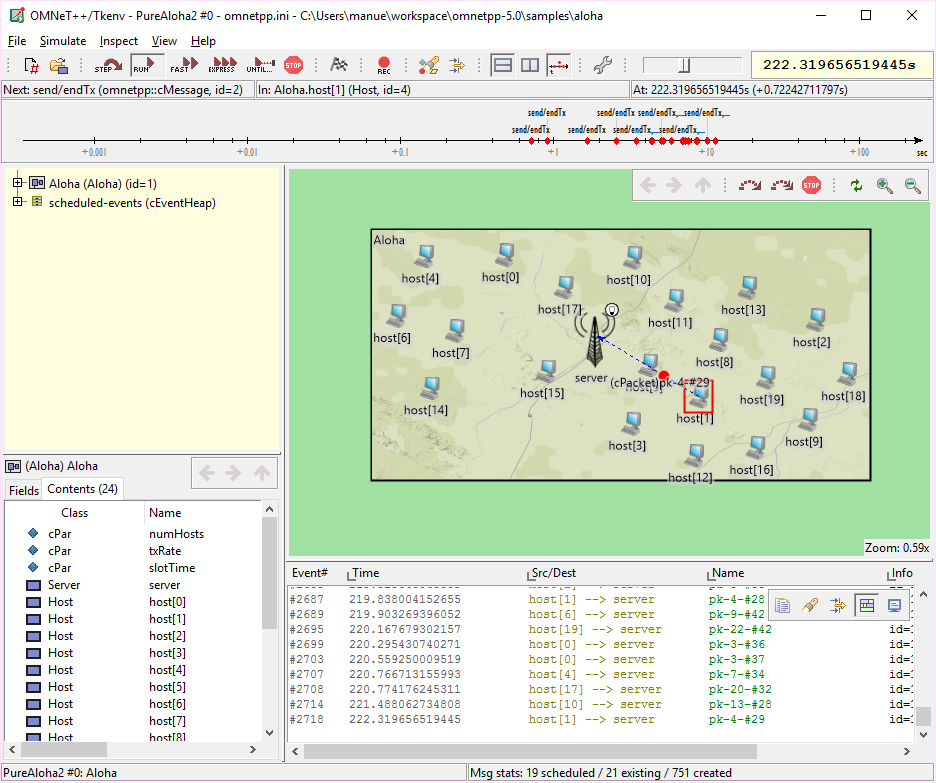
\includegraphics[width=.8\linewidth]{figuras/omnetpp_aloha}
    \caption{Entorno de simulación gráfica de OMNeT++.}
    \label{fig:omnetpp_simgui}
\end{figure}

OMNeT++, \emph{\textbf{O}bjective \textbf{M}odular \textbf{Ne}twork \textbf{T}estbed in C\textbf{++}}, es un entorno modular y basado en componentes para la simulación de sistemas de eventos discretos \cite{omnet2008overview}. Está escrito en C++, y si bien en estricto rigor OMNeT++ en sí sólo conforma el \emph{framework} genérico para la definición de modelos, la distribución incluye además múltiples extensiones para el modelamiento de redes de comunicación -- siendo la principal de éstas INET.

INET incluye modelos para la simulación de múltiples \emph{stacks} de protocolos para la comunicación tanto cableada como inalámbrica, a través de una gran cantidad de protocolos (IPV6, WSN, etc.). Finalmente, INET incluye además modelos de movilidad, para el estudio de redes con nodos en movimiento.

OMNeT++ presenta una gran ventaja en su diseño modular y extensible, y se posiciona como una excelente opción para simulaciones que requieran un alto nivel de flexibilidad.

\subsubsection{ns-2 y ns-3}

ns-2 es un simulador de eventos discretos para la simulación de redes de comunicación, cuyo desarrollo comenzó en 1989 y que a lo largo de los años ha recibido grandes contribuciones tanto de la comunidad científico como de corporaciones como DARPA, Xerox, etc. Gracias a su larga trayectoria y extenso soporte, actualmente cuenta con un gran renombre en academia.

El simulador y sus módulos en sí están escritos en C++, pero se utiliza una extensión del lenguaje Tcl para su configuración y la definición de topologías de red. Esta decisión de diseño fue producto de un deseo de evitar la recompilación del simulador al realizar cambios en algún escenario, lo cual tenía mucho sentido en un tiempo en que la compilación implicaba extensos tiempos de espera. Hoy en día sin embargo, con los avances en potencia computacional, es más una desventaja, perjudicando la escalabilidad del sistema \autocite{perf_comp_recentnetworksims} a cambio de una marginal mejora en tiempos de recompilación. 

ns-3 es considerado el sucesor de ns-2, llevando el exitoso simulador al siglo XXI. A diferencia de su ancestro, ns-3 está escrito completamente en C++, y opcionalmente algunos módulos pueden definirse en Python. Además, ns-3 incluye extensas optimizaciones en términos de escalabilidad y paralelismo, a cambio de una incompatibilidad con antiguos modelos desarrollados para ns-2

\subsection{Entornos de simulación bidireccional}

A continuación se resumirá brevemente el estado del arte en el tema de simulación bidireccional para simulaciones de Sistemas Inteligentes de Transporte. 

\subsubsection{Simulaciones unidireccionales}

De acuerdo a Sommer \emph{et al.} \autocite{bidirectionalsimul}, la mayor parte de las simulaciones de comunicaciones inalámbricas en ITS se hacen a través de la importación de trazas de movimiento reales desde simuladores de transporte, de manera unidireccional. Dichas trazas se pueden generar de dos manera: \textit{offline}, es decir, aisladamente en el simulador de transporte, para luego ser exportadas en un formato que el simulador de red sea capaz de interpretar, y \textit{decoupled online}, de manera que el simulador de transporte genere las trazas en tiempo real y el simulador de red simplemente las ``consume''. Sin embargo, si bien este método permite analizar el efecto del modelo de movimiento de un sistema de transporte en las comunicaciones inalámbricas, es incapaz de reflejar el impacto de la propagación de información del estado del tráfico en el modelo mismo. Es decir, esta metodología no es útil para la simulación de, por ejemplo, sistemas de advertencia de accidentes o de asistencia al conductor, puesto que las trazas de movimiento están predefinidas o se generan sin considerar los resultados de esta comunicación. Este tipo de simulación, si bien es útil para ciertos análisis específicos, no constituye una simulación bidireccional y no abarca la totalidad del problema.

Los trabajos realizados por investigadores de la Universidad Jiao Tong de Shanghai en \autocite{suvnet1,suvnet2} son ejemplos de esta modalidad. Para estas investigaciones, los autores obtuvieron trazas reales de movimiento de SUVnet, una red vehicular compuesta por aproximadamente 4000 taxis en la ciudad de Shanghai. Estas trazas luego fueron simplemente utilizadas en simulaciones de red de comunicaciones para la validación de los modelos desarrollados.

Otro ejemplo de esto es la investigación presentada por Goebel \emph{et al.} en \autocite{omnetv2xtraces}. En este trabajo, los investigadores utilizaron SUMO para la generación de trazas vehiculares realistas, las cuales luego fueron importadas en OMNeT++ para el estudio del impacto de la movilidad vehicular en comunicaciones celulares. 

\subsubsection{Entornos integrados}\label{sec:integrated_sim}

\begin{figure}
    \centering
    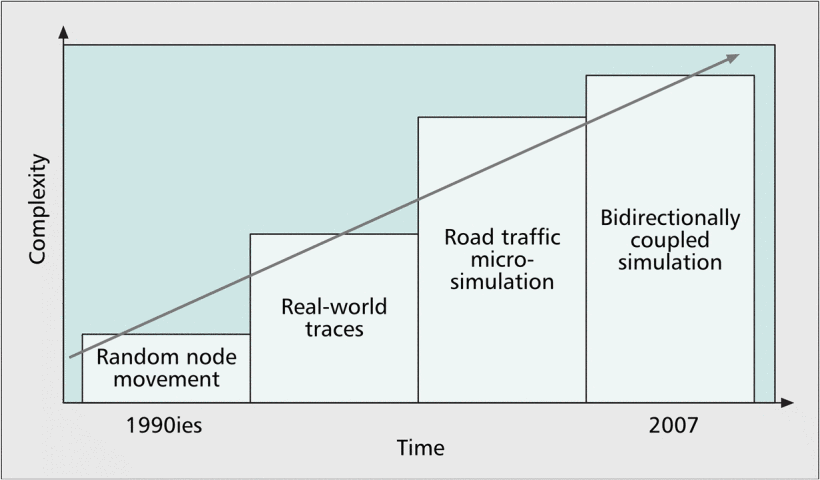
\includegraphics[width=\linewidth]{figuras/evolution_bidirectional_sim_sommerdressler.png}
    \caption[Evolución de simulaciones integradas.]{Evolución de simulaciones integradas para ITS (fuente: Sommer y Dressler \autocite{sommer_dressler2}).}
    \label{fig:bidir_evol}
\end{figure}

La necesidad de un entorno integrado para la simulación de Sistemas Inteligentes de Transportes es un tema que ha estado presente en la comunidad académica hace casi más de una década ya. En particular, Sommer \emph{et al.} argumentaron fuertemente a favor de la idea en \autocite{bidirectionalsimul} y \autocite{sommer_dressler2}; el siguiente análisis se basa principalmente en ambos documentos, con algunas fuentes adicionales que se mencionarán oportunamente. 

En primer lugar, los autores destacan la existencia de un sistema de simulación bidireccional desarrollado por la Universidad Nacional de Chiao Tung, Taiwan \autocite{nctuns4,nctuns6}, el cual permite la simulación íntegra de un sistema de transportes dotado de capacidades de comunicación inalámbrica. 

NCTUns, actualmente en su versión 6.0 (publicada en junio del 2010 \autocite{nctuns6}), es un simulador para el estudio de Sistemas Inteligentes de Transporte. Su principal particularidad es que presenta un entorno totalmente integrado para la ejecución de dichas simulaciones; es decir, es tanto un simulador de redes de comunicaciones como de tráfico. Incluye capacidades para simular comportamiento tanto autónomo como predefinido (\emph{rutas}) de vehículos, e implementa un \emph{stack} de protocolo completo en cada vehículo.

No obstante, Sommer \emph{et al.} critican la incompatibilidad de dicho sistema (en su versión 4.0) con los modelos de protocolos de comunicación y transporte ya desarrollados para los simuladores más prominentes, limitando su utilidad práctica en la investigación. Además. si bien NCTUns es capaz de simular un número capacidad de capas físicas, todavía se encuentra muy limitado en ese aspecto en comparación con otros simuladores de redes.

Los investigadores mencionan también la existencia de TraNS \autocite{piorkowski2008trans}, un \emph{framework} para la integración de ns-2 con SUMO. Este sistema implementa un \emph{loop} de control y \emph{feedback} activo entre ambos simuladores, estableciendo así una simulación bidireccional que permite la emulación de un ITS.

TraNS integra dos simuladores de renombre en la academia, y ha sido muy bien recibido. Sin embargo, los autores destacan que carece de ciertas funcionalidades -- principalmente, la capacidad de sincronizar y controlar el tiempo de simulación entre ambos simuladores.

Se debe destacar también los trabajos realizados por investigadores en la Universidad Estatal de Nueva York en Buffalo \autocite{zhao2016integrated} y de la Universidad de Düsseldorf \autocite{lochert2005multiple}. Ambos constituyen ejemplos de simulaciones bidireccionales -- no obstante se ven limitados por su especificidad, y dificultad de adaptación a escenarios más diversos. El trabajo de Shalaby en su tesis de magíster \autocite{shalaby} también sufre este mismo problema, además de temas relacionados a la eficiencia del \emph{framework} desarrollado por la autora, principalmente ligados a la elección de mecanismo de comunicación entre los simuladores (archivos en disco).


Finalmente, Sommer, German y Dressler presentan su solución en \autocite{sommer_german_dressler}: VEINS, un \textit{framework} de integración entre OMNeT++ y SUMO. Ambos simuladores se escogieron específicamente por su adopción en el mundo académico, y por sus naturalezas abiertas y fáciles de adaptar y modificar.

A través de VEINS, ambos simuladores se ejecutan en paralelo, comunicándose en tiempo real mediante un \textit{socket} utilizando el protocolo TCP; SUMO proporciona las trazas de movimiento de los elementos en la simulación a la vez que OMNeT++ simula el comportamiento de la red de comunicaciones. Además, mediante este esquema, OMNeT++ también puede modificar directamente el comportamiento del modelo de transporte, por ejemplo alterando la velocidad de un vehículo en respuesta a un mensaje específico obtenido a través de la red de comunicaciones. De esta manera, el \textit{framework} en cuestión permite modelar sistemas complejos y dinámicos, que reflejan de buena manera la realidad.

Sin embargo, VEINS sufre por su elección de simulador de transporte; SUMO todavía se encuentra en una temprana etapa de desarrollo, lo cual implica que frecuentemente sufre de problemas de estabilidad y de falta de características y documentación. Por ejemplo, hasta diciembre del 2015 (versión 0.25.0), SUMO no contaba con un editor gráfico de redes de transporte\footnote{\url{http://sumo.dlr.de/wiki/FAQ}}, lo cual dificultaba mucho el diseño de redes originales. Además, la curva de aprendizaje de SUMO es bastante pronunciada, y todas sus configuraciones son a través de archivos; es por esto que en muchos departamentos de ingeniería de transporte se opta por otros simuladores más avanzados y estables. 


